
\documentclass[11pt, class=report,crop=false]{standalone}
\usepackage[screen]{exo7book}


\begin{document}

%====================================================================
\chapitre{Extremums}
%====================================================================

% A garder
%\DeclareMathOperator{\grad}{grad}  % dans le préambule
\newcommand{\grad}{\operatorname{grad}} % dans le document

\newcommand{\myscale}{1}

%%%%%%%%%%%%%%%%%%%%%%%%%%%%%%%%%%%%%%%%%%%%%%%%%%%%%
\section{Motivation -- Cas d'une variable}



Comment trouver le maximum (ou le minimum) d'une fonction $f : \Rr^n  \to \Rr$ ?
Ce chapitre est consacré à l'étude de l'existence des extremums.
Nous apprendrons à repérer les extremums locaux (qui ne sont pas nécessairement des minimums ou maximums globaux). 
On terminera ce chapitre par l'étude des \og{}extremums liés\fg{},
où la recherche est limitée par une contrainte.
Pour mieux comprendre ce qui se passe en plusieurs variables, on commence par revoir rapidement le cas d'une variable.

%----------------------------------------------------
\subsection{Minimum, maximum, point critique}

Soit $f : \Rr \to \Rr$ une fonction d'une variable.
\begin{itemize}
      \item $f$ admet un \defi{maximum local} en $x_0 \in \Rr$ s'il existe un intervalle ouvert $I$ contenant $x_0$ tel que :
      $$\text{pour tout } x \in I \qquad f(x) \le f(x_0).$$
      
      \item $f$ admet un \defi{minimum local} en $x_0 \in \Rr$ s'il existe un intervalle ouvert $I$ contenant $x_0$ tel que :
$$\text{pour tout } x \in I \qquad f(x) \ge f(x_0).$$ 

      \item $f$ admet un \defi{extremum local} en $x_0 \in \Rr$ si $f$ admet un maximum local ou bien un minimum local en ce point.
      \item $f$ admet un \defi{point critique} en $x_0 \in \Rr$ si $f'(x_0)=0$. Géométriquement, c'est un point de tangente horizontale.
      
      \item Proposition : si $f$ dérivable admet un minimum local ou un maximum local en $x_0$, alors $f'(x_0)=0$.
      Autrement dit, si $x_0$ est un extremum local alors c'est un point critique.
      
      \item La réciproque n'est pas toujours vraie. Par exemple, pour $f: x \mapsto x^3$, le point $x_0=0$ est un point critique, mais ce n'est ni un maximum local ni un minimum local (c'est un \defi{point d'inflexion}).
      
   
\end{itemize}


\myfigure{1}{
    \tikzinput{fig-extrem-01}\qquad 
    \tikzinput{fig-extrem-02}    
}
Sur la figure de gauche : des exemples de minimum local, maximum local, maximum global ; il n'y a pas de minimum global sur $\Rr$. Sur la figure de droite : un extremum local est nécessairement un point critique.

%----------------------------------------------------
\subsection{Exemples fondamentaux}

\begin{itemize}
    \item $f : x \mapsto x^2$, minimum local en $0$, on a $f'(0)=0$ et $f''(0)>0$.
    \item $f : x \mapsto -x^2$, maximum local en $0$, on a $f'(0)=0$ et $f''(0)<0$.
    \item $f : x \mapsto x^3$, ni minimum ni maximum local en $0$, on a $f'(0)=0$ et $f''(0)=0$.      
\end{itemize}

\myfigure{1}{
    \tikzinput{fig-extrem-03a}\qquad\qquad
    \tikzinput{fig-extrem-03b}\qquad\qquad
    \tikzinput{fig-extrem-03c}        
}

%----------------------------------------------------
\subsection{Formule de Taylor à l'ordre 2}

Soit $f : \Rr \to \Rr$ une fonction d'une variable de classe $\mathcal{C}^2$. 
\begin{theoreme}[Formule de Taylor à l'ordre $2$] 
Pour tout $x_0 \in \Rr$, on a
\mybox{$f(x_0 + h) = f(x_0) + hf'(x_0) + \frac{h^2}{2} f''(x_0) + h^2 \epsilon(h)$}
où $\epsilon(h) \to 0$ lorsque $h\to0$.
\end{theoreme}

Le développement limité à l'ordre $1$, $f(x_0 + h) \simeq f(x_0) + hf'(x_0)$, correspond à l'approximation du graphe de $f$ par sa tangente en $x_0$ (figure de gauche ci-dessous).
Le développement limité à l'ordre $2$, $f(x_0 + h) \simeq f(x_0) + hf'(x_0) + \frac{h^2}{2} f''(x_0)$, correspond à une approximation par une parabole (figure de droite).


\myfigure{0.7}{
    \tikzinput{fig-extrem-04a}\qquad \qquad 
    \tikzinput{fig-extrem-04b}    
}


Choisissons pour $x_0$ une valeur telle que $f'(x_0)=0$ et $f''(x_0)\neq 0$. 
Alors, pour $h$ assez petit, le terme $ \frac{h^2}{2} f''(x_0) + h^2 \epsilon (h)$ est du même signe que $f''(x_0)$. Si par exemple $f''(x_0)>0$, on en déduit que $f(x_0 + h) \ge f(x_0)$ (pour $h$ proche de $0$) et donc que $f$ admet un minimum local en $x_0$.
Ci-dessous, on va en déduire une caractérisation des minimums et maximums.

%----------------------------------------------------
\subsection{Caractérisation des minimums et maximums}

La recherche pratique des extremums locaux pour une fonction d'une variable se passe donc ainsi :
\begin{enumerate}
    \item On recherche les points critiques donnés par l'équation $f'(x) = 0$.
    \item Pour chaque point critique $x_0$, on calcule la dérivée seconde :
    \begin{itemize}
        \item si $f''(x_0) > 0$, alors $f$ admet un minimum local en $x_0$,   
        \item si $f''(x_0) < 0$, alors $f$ admet un maximum local en $x_0$,
        \item si $f''(x_0) = 0$, alors  il faut approfondir l'étude.
    \end{itemize}    
\end{enumerate}
    
Lorsque $f : [a,b] \to \Rr$ est définie sur un intervalle compact, il faudra en plus étudier le comportement de $f$ en $a$ et en $b$ (c'est-à-dire au bord du domaine de définition). Comme l'ensemble de départ est compact, on a la garantie de l'existence d'extremums globaux.
    

%%%%%%%%%%%%%%%%%%%%%%%%%%%%%%%%%%%%%%%%%%%%%%%%%%%%%
\section{Dérivées partielles d'ordre 2}

%----------------------------------------------------
\subsection{Dérivées partielles d'ordre 2}

Soit $f : \Rr^2 \to \Rr$ une application différentiable.
Les deux dérivées partielles $\frac{\partial f}{\partial x}$
et $\frac{\partial f}{\partial y}$ sont aussi des fonctions de $\Rr^2$ dans $\Rr$ ; 
supposons que ce soient aussi des applications différentiables.
Alors on peut calculer les dérivées partielles de $\frac{\partial f}{\partial x}$ :
$$\frac{\partial}{\partial x}\left(\frac{\partial f}{\partial x}\right)
\qquad \text{ et } \qquad 
\frac{\partial}{\partial y}\left(\frac{\partial f}{\partial x}\right).$$
On peut aussi calculer les dérivées partielles de $\frac{\partial f}{\partial y}$ :
$$\frac{\partial}{\partial x}\left(\frac{\partial f}{\partial y}\right)
\qquad \text{ et } \qquad 
\frac{\partial}{\partial y}\left(\frac{\partial f}{\partial y}\right).$$

On note ces dérivées partielles :
$$\frac{\partial ^2 f}{\partial x^2}
\qquad
\frac{\partial ^2 f}{\partial y\partial x}
\qquad
\frac{\partial ^2 f}{\partial x\partial y}
\qquad
\frac{\partial ^2 f}{\partial y^2}
$$
Ce sont des fonctions de $\Rr^2$ dans $\Rr$.


Plus généralement, pour $f : \Rr^n \to \Rr$, on note $\frac{\partial f}{\partial x_i} : \Rr^n \to \Rr$ les dérivées partielles d'ordre $1$ ($1 \le i \le n$)
et $\frac{\partial ^2f}{\partial x_j\partial x_i}$ les dérivées partielles d'ordre $2$ ($1 \le i,j \le n$).


%----------------------------------------------------
\subsection{Théorème de Schwarz}


Pour $f : \Rr^2 \to \Rr$, il y a quatre dérivées partielles secondes à calculer, mais en général deux d'entre elles sont égales.

\begin{exemple}
Soit $f : U \to \Rr$ définie par $f(x,y) = x^2\cos(y) + \ln(x-y^2)$ sur $U = \big\{ (x,y) \in \Rr^2 \mid x-y^2>0 \big\}$.
Alors :
$$\frac{\partial f}{\partial x}(x,y) = 2x\cos(y) + \frac{1}{x-y^2}
\qquad\qquad
\frac{\partial f}{\partial y}(x,y) = -x^2\sin(y) - \frac{2y}{x-y^2}$$

On peut maintenant dériver une nouvelle fois pour obtenir les dérivées partielles d'ordre $2$ :
$$\frac{\partial ^2 f}{\partial x^2}(x,y) 
= \frac{\partial}{\partial x}\left(\frac{\partial f}{\partial x}(x,y)\right)
= \frac{\partial}{\partial x}\left(2x\cos(y) + \frac{1}{x-y^2}\right)
= 2\cos(y) - \frac{1}{(x-y^2)^2}$$

$$\frac{\partial ^2 f}{\partial y\partial x}(x,y) 
= \frac{\partial}{\partial y}\left(\frac{\partial f}{\partial x}(x,y)\right)
= \frac{\partial}{\partial y}\left(2x\cos(y) + \frac{1}{x-y^2}\right)
= \boxed{-2x\sin(y) + \frac{2y}{(x-y^2)^2}}$$

$$\frac{\partial ^2 f}{\partial x\partial y}(x,y) 
= \frac{\partial}{\partial x}\left(\frac{\partial f}{\partial y}(x,y)\right)
= \frac{\partial}{\partial x}\left(-x^2\sin(y) - \frac{2y}{x-y^2}\right)
= \boxed{-2x\sin(y) + \frac{2y}{(x-y^2)^2}}$$

$$\frac{\partial ^2 f}{\partial y^2}(x,y) 
= \frac{\partial}{\partial y}\left(\frac{\partial f}{\partial y}(x,y)\right)
= \frac{\partial}{\partial y}\left(-x^2\sin(y) - \frac{2y}{x-y^2}\right)
= -x^2\cos(y) - \frac{2x+2y^2}{(x-y^2)^2}$$


\end{exemple}

On note sur l'exemple précédent que $\frac{\partial ^2 f}{\partial y\partial x}(x,y) = \frac{\partial ^2 f}{\partial x\partial y}(x,y)$. C'est un phénomène général que l'on va détailler.


\begin{definition}
    Une fonction $f : \Rr^n \to \Rr$ est de \defi{classe $\mathcal{C}^2$} si $f$ est de classe $\mathcal{C}^1$ (c'est-à-dire ses dérivées partielles existent et sont continues) et si ses dérivées partielles sont aussi de classe $\mathcal{C}^1$.
\end{definition}

Le théorème de Schwarz dit que le résultat ne dépend pas de l'ordre dans lequel on effectue les dérivations.
\begin{theoreme}[Théorème de Schwarz]
Soit $f:U\subset \Rr^n\to \Rr$ une fonction de classe $\mathcal{C}^2$. 
Pour tous $i,j  \in \{1,\dots ,n\}$, on a :
    \mybox{$\displaystyle \frac{\partial}{\partial x_i}\left(\frac{\partial f}{\partial x_j}\right)=\frac{\partial}{\partial x_j}\left(\frac{\partial f}{\partial x_i}\right)$}
\end{theoreme}

Ainsi, pour $f : \Rr^2 \to \Rr$ de classe $\mathcal{C}^2$, on a :
\mybox{$\displaystyle \frac{\partial ^2 f}{\partial y\partial x}(x,y) = \frac{\partial ^2 f}{\partial x\partial y}(x,y)$}

Pour $f : \Rr^3 \to \Rr$ de classe $\mathcal{C}^2$, il y a $9$ dérivées partielles d'ordre $2$, mais seulement $6$ calculs à faire :
 $$\frac{\partial ^2 f}{\partial x^2}
 \qquad
 \frac{\partial ^2 f}{\partial y^2}
 \qquad
 \frac{\partial ^2 f}{\partial z^2}  
 \qquad 
 \frac{\partial ^2 f}{\partial y\partial x}= \frac{\partial ^2 f}{\partial x\partial y}
 \qquad
 \frac{\partial ^2 f}{\partial z\partial x}= \frac{\partial ^2 f}{\partial x\partial z}
 \qquad
 \frac{\partial ^2 f}{\partial z\partial y}= \frac{\partial ^2 f}{\partial y\partial z} 
 $$


Le contre-exemple suivant, qui peut être omis lors d'une première lecture, prouve qu'il est nécessaire d'avoir une fonction de classe $\mathcal{C}^2$. Si cette hypothèse manque alors les dérivées partielles croisées peuvent ne pas être égales.

\begin{exemple}
Soit $f: \Rr^2 \to \Rr$ la fonction définie par
$$f(x,y)=\frac{xy^3}{x^2+y^2}\;\mbox{ si }(x,y)\neq (0,0)\quad \mbox{et}\quad f(0,0)= 0.$$
On vérifie que $f$ est de classe $\mathcal{C}^1$ sur $\Rr^2$ et que
$$\frac{\partial f}{\partial x}(x,y)=\left\{\begin{array}{cl}\displaystyle \frac{y^5-x^2y^3}{(x^2+y^2)^2}&\mbox{si }(x,y)\neq (0,0)\\ 0&\mbox{si }(x,y)=(0,0)
\end{array}\right.$$
et 
$$\frac{\partial f}{\partial y}(x,y)=\left\{\begin{array}{cl}\displaystyle \frac{3x^3y^2+xy^4}{(x^2+y^2)^2}&\mbox{si }(x,y)\neq (0,0)\\ 0&\mbox{si }(x,y)=(0,0).\end{array}\right.$$
Le taux d'accroissement
$$\frac{\frac{\partial f}{\partial x}(0,y)-\frac{\partial f}{\partial x}(0,0)}{y-0}=1\underset{y\to 0\; \; \; }{\longrightarrow 1}$$
ce qui montre que $\displaystyle \frac{\partial ^2f}{\partial y\partial x}(0,0)=1$.
De même, le taux d'accroissement
$$\frac{\frac{\partial f}{\partial y}(x,0)-\frac{\partial f}{\partial y}(0,0)}{x-0}=0\underset{x\to 0\; \; \; }{\longrightarrow 0}$$
ce qui montre que $\displaystyle \frac{\partial ^2f}{\partial x\partial y}(0,0)=0$. 
Les dérivées partielles croisées ne sont pas égales en $(0,0)$.
On en déduit que l'une (au moins) des dérivées partielles secondes $\displaystyle \frac{\partial ^2f}{\partial x\partial y}$ ou $\displaystyle \frac{\partial ^2f}{\partial y\partial x}$ n'est pas continue en $(0,0)$. Autrement dit, la fonction $f$ n'est pas de classe $\mathcal{C}^2$ en $(0,0)$ et le théorème de Schwarz ne s'applique pas.
\end{exemple}


%----------------------------------------------------
\subsection{Hessienne}

La matrice jacobienne est la matrice des dérivées partielles.
La matrice hessienne est la matrice des dérivées partielles d'ordre $2$.

Soit $f : \Rr^n \to \Rr$ une fonction de $n$ variables.
La \defi{matrice hessienne} de $f$ en $x=(x_1,\ldots,x_n)$ est la matrice $n \times n$ :
\mybox{$\displaystyle H_f(x) = \left( \frac{\partial ^2f}{\partial x_i\partial x_j}(x) \right)_{1 \le i,j \le n}$}
Pour une fonction de classe $\mathcal{C}^2$, d'après le théorème de Schwarz, c'est une \evidence{matrice symétrique}.


Dans le cas d'une fonction de deux variables :
\mybox{$\displaystyle 
H_f(x,y)
 = 
\begin{pmatrix}
\frac{\partial ^2f}{\partial x^2}(x,y) & \frac{\partial ^2f}{\partial x\partial y}(x,y) \\
\frac{\partial ^2f}{\partial y\partial x}(x,y) & \frac{\partial ^2f}{\partial y^2}(x,y) \\
\end{pmatrix}$}
% = 
%\begin{pmatrix}
%r(x,y) & s(x,y) \\
%s(x,y) & t(x,y) \\
%\end{pmatrix}
%$$

\bigskip

Pour trois variables, la matrice hessienne (à évaluer en $(x,y,z)$) vaut :
$$H_f=
\begin{pmatrix}
\frac{\partial^2f}{\partial x^2}&\frac{\partial^2f}{\partial x\partial y}&\frac{\partial^2f}{\partial x\partial z}\\  \frac{\partial^2f}{\partial y\partial x}&\frac{\partial^2f}{\partial y^2}&\frac{\partial^2f}{\partial y\partial z}\\  \frac{\partial^2f}{\partial z\partial x}&\frac{\partial^2f}{\partial z\partial y}&\frac{\partial^2f}{\partial z^2}\\
\end{pmatrix}.$$

\begin{exemple}
Calculons la matrice hessienne de $f(x,y) = xy^2 + x^4 - y^4$.

On calcule d'abord 
$$\frac{\partial f}{\partial x}(x,y) = 4x^3 + y^2
\qquad\qquad
\frac{\partial f}{\partial y}(x,y) = 2xy - 4y^3.$$

On a donc 
$$H_f(x,y)
= \begin{pmatrix}
    \frac{\partial ^2f}{\partial x^2}(x,y) & \frac{\partial ^2f}{\partial x\partial y}(x,y) \\
    \frac{\partial ^2f}{\partial y\partial x}(x,y) & \frac{\partial ^2f}{\partial y^2}(x,y) \\
\end{pmatrix}
= 
\begin{pmatrix}
12x^2 & 2y \\
2y      & 2x - 12y^2 \\
\end{pmatrix}.$$
\end{exemple}


%----------------------------------------------------
\begin{miniexercices}
    \sauteligne
    \begin{enumerate}
        \item Soit $f(x,y) = x^3+5x^2y-y^2$. Calculer les dérivées partielles d'ordre $1$ de $f$. Calculer les dérivées partielles d'ordre $2$ de $f$. Vérifier la validité du théorème de Schwarz. Calculer la matrice hessienne de $f$. Calculer les dérivées partielles d'ordre $3$ de $f$.
        
        \item Soit $f(x,y) = xe^{x^2-y^2}$. Calculer les dérivées partielles d'ordre $1$ et d'ordre $2$ de $f$. Calculer la matrice hessienne de $f$.
        
        \item Soit $f(x,y,z) = xy^2 \ln(z)$. Déterminer l'ensemble de définition de $f$. Calculer les dérivées partielles d'ordre $1$ et d'ordre $2$ ainsi que la matrice hessienne de $f$.                
    \end{enumerate}
\end{miniexercices}


%%%%%%%%%%%%%%%%%%%%%%%%%%%%%%%%%%%%%%%%%%%%%%%%%%%%%
\section{Formule de Taylor à l'ordre 2}

%----------------------------------------------------
\subsection{Formule de Taylor à l'ordre 1}

Nous avons déjà vu qu'une façon de dire que $f$ est différentiable est de dire que $f$ admet un \defi{développement limité à l'ordre $1$}. Pour $f : \Rr^2 \to \Rr$,
au point $(x_0,y_0)$, si $f$ est différentiable alors
$$f(x_0+h,y_0+k)=f(x_0,y_0)+h\frac{\partial f}{\partial x}(x_0,y_0)+k\frac{\partial f}{\partial y}(x_0,y_0)+o\left(\|(h,k)\|\right).$$

Connaissant les valeurs de $f$, $\frac{\partial f}{\partial x}$
et $\frac{\partial f}{\partial y}$ uniquement en $(x_0,y_0)$, on en déduit une approximation de $f$ en tout $(x,y)$ proche de $(x_0,y_0)$.

\medskip

Le but va être d'améliorer cette approximation par un développement limité à l'ordre $2$.

On rappelle la notation \og{}petit o\fg{}.

\textbf{Notation.} Soit $g :\Rr^2\to \Rr$ une fonction définie au voisinage de $(0,0)$. On dit que $g$ est \defi{négligeable} par rapport à $\|(x,y)\|^n$ au voisinage de $(0,0)$ et on note $g=o\left(\|(x,y)\|^n\right)$ si 
$$\lim_{(x,y)\to(0,0)}\frac{g(x,y)}{\|(x,y)\|^n}=0.$$

\textbf{Interprétation géométrique.}

Le plan tangent (en bleu) au graphe de $f$ au point $(x_0,y_0)$ est le plan qui approche le mieux le graphe de $f$ (en rouge) autour de ce point.
Pour calculer $f(x,y)$ lorsque $(x,y)=(x_0+h,y_0+k)$ est proche de $(x_0,y_0)$, on remplace la valeur exacte $z_{exact} = f(x,y)$ 
par son approximation $z_{approx} = f(x_0,y_0)+h\frac{\partial f}{\partial x}(x_0,y_0)+k\frac{\partial f}{\partial y}(x_0,y_0)$.
Le point $(x,y,z_{exact})$ est un point du graphe de $f$ alors que
$(x,y,z_{approx})$ est un point du plan tangent au graphe de $f$ au point $(x_0,y_0)$. 


 \myfigure{1}{
     \tikzinput{fig-extrem-06}        
 }


%----------------------------------------------------
\subsection{Formule de Taylor à l'ordre 2 (en 2 variables)}

\begin{theoreme}    
Soit $f:U \to \Rr$ une fonction de classe $\mathcal{C}^2$ sur un ouvert $U\subset \Rr^2$ et soit $(x_0,y_0)\in U$.  Alors :
\mybox{\begin{align*}
f(x_0+h,y_0+k) 
& = f(x_0,y_0)
\ + \  h\frac{\partial f}{\partial x}(x_0,y_0)
+k\frac{\partial f}{\partial y}(x_0,y_0) \\
& \qquad +\frac{1}{2}\left[
h^2\frac{\partial ^2f}{\partial x^2}(x_0,y_0)
+2hk\frac{\partial ^2f}{\partial x\partial y}(x_0,y_0)
+k^2\frac{\partial ^2f}{\partial y^2}(x_0,y_0)
\right] \\ 
& \qquad \qquad +o\left(\|(h,k)\|^2\right)
\end{align*}}
   
\end{theoreme}


\begin{itemize}
    \item On dit aussi que $f$ admet un développement limité d'ordre $2$ au point $(x_0,y_0)$.

    \item Attention à ne pas oublier le facteur $\frac12$ devant les termes de degré $2$, ni le facteur $2$ devant le terme $hk$.
    
    \item On rappelle que si on choisit la norme euclidienne alors $\|(h,k)\|^2 = h^2+k^2$ et que $o\left(\|(h,k)\|^2\right)$ désigne une fonction égale à $\|(h,k)\|^2 \epsilon(h,k)$ avec $\epsilon(h,k) 
    \xrightarrow[(h,k)\to (0,0)]{} 0.$


\end{itemize}



\begin{exemple}
Étudions $f(x,y) = \exp(xy^2-2)$ autour de $(x_0,y_0) = (2,1)$.
\begin{itemize}
    \item $f(2,1) = 1$.
    
    \item \textbf{DL à l'ordre 1.}
    $$\frac{\partial f}{\partial x}(x,y) = y^2\exp(xy^2-2)
    \quad
    \frac{\partial f}{\partial y}(x,y) = 2xy\exp(xy^2-2)
    \quad\text{ donc }\quad
    \frac{\partial f}{\partial x}(2,1) = 1
    \quad
    \frac{\partial f}{\partial y}(2,1) = 4$$
    Ainsi :
    $$f(2+h,1+k) = 1 + h + 4k + o\left(\|(h,k)\|\right).$$
  
    \item \textbf{DL à l'ordre 2.} 
    
    \begin{align*}
    \frac{\partial ^2f}{\partial x^2}(x,y) &= y^4\exp(xy^2-2) \\
    \frac{\partial ^2f}{\partial x\partial y}(x,y) &= (2y+2xy^3)\exp(xy^2-2)\\
    \frac{\partial ^2f}{\partial y^2}(x,y) &= (2x+4x^2y^2)\exp(xy^2-2)
    \end{align*}
    Donc :
    $$\frac{\partial ^2f}{\partial x^2}(2,1) = 1\qquad 
    \frac{\partial ^2f}{\partial x\partial y}(2,1) = 6 \qquad
    \frac{\partial ^2f}{\partial y^2}(2,1) = 20.$$ 
    Ainsi :
    $$   
    f(2+h,1+k)  \ 
    = \  1 \quad + \quad h + 4k
    \quad +\quad
    \frac12\left(h^2
    +2\cdot 6 \cdot hk
    +20 k^2\right)
    \quad + \quad o\left(\|(h,k)\|^2\right).$$

\end{itemize}    
       
\end{exemple}    



\bigskip

\textbf{Interprétation géométrique.}
Un développement limité à l'ordre $1$ correspond à approcher le graphe de $f$ par un plan tangent d'équation $z=a +bx+cy$. 
Un développement limité à l'ordre $2$ correspond à une approximation par une surface quadratique, c'est-à-dire une surface définie par une équation de degré $2$ :
$$z=a +bx+cy + dx^2 + 2exy + fy^2.$$
Cette approximation est meilleure mais reste valable uniquement autour du point $(x_0,y_0)$ considéré.


\bigskip

\textbf{Approximations numériques.}

Si $(x,y)$ est proche de $(x_0,y_0)$ (c'est-à-dire si $h$ et $k$ sont petits), alors on remplace le calcul de $f(x,y)$ qui peut être compliqué par une bonne approximation donnée par le DL à l'ordre $1$, ou mieux, le DL à l'ordre $2$.

\begin{exemple}
Sans calculatrice, évaluons $\sqrt{1+x+xy}$ avec $x=0.1$ et $y=0.2$.

Soit $f(x,y) = \sqrt{1+x+xy} = (1+x+xy)^{\frac12}$ que l'on étudie autour de $(x_0,y_0)=(0,0)$.
Alors :
\begin{itemize}
    \item $f(0,0) = 1$.
    
    \item \textbf{DL à l'ordre 1.}
    $$\frac{\partial f}{\partial x}(x,y) = \frac{1+y}{2}(1+x+xy)^{-\frac12}
    \qquad\qquad
    \frac{\partial f}{\partial y}(x,y) = \frac{x}{2}(1+x+xy)^{-\frac12}$$
    donc
    $$\frac{\partial f}{\partial x}(0,0) = \frac12
    \qquad\qquad
    \frac{\partial f}{\partial y}(0,0) = 0.$$
    Ainsi, pour $(x,y)$ proche de $(0,0)$, on a  
    $$f(x,y) \simeq 1+\frac12x.$$ 
      
    \item \textbf{DL à l'ordre 2.} 
    
    \begin{align*}
    \frac{\partial^2f}{\partial x^2}(x,y) &=  -\frac{(1+y)^2}{4}(1+x+xy)^{-\frac32}\\
    \frac{\partial^2f}{\partial x\partial y}(x,y) &= \frac{2+x+xy}{4}(1+x+xy)^{-\frac32}\\
    \frac{\partial^2f}{\partial y^2}(x,y) &= -\frac{x^2}{4}(1+x+xy)^{-\frac32}
    \end{align*}
    donc 
    $$\frac{\partial^2f}{\partial x^2}(0,0) = -\frac14\qquad \qquad
    \frac{\partial^2f}{\partial x\partial y}(0,0) = \frac12 \qquad\qquad
    \frac{\partial^2f}{\partial y^2}(0,0) = 0.$$ 
    Ainsi, pour $(x,y)$ proche de $(0,0)$, on a 
    $$   
    f(x,y) 
    \simeq \ 1 \  + \  \frac12x
    \  +\ 
    \frac12\left(-\frac14x^2+ xy\right).
    $$
    
      
\item \textbf{Valeurs numériques.}
    Avec $x=0.1$ et $y=0.2$, la valeur exacte est $f(x,y) = \sqrt{1.12} = 1.05830\,\ldots$
    Le DL à l'ordre $1$ fournit l'approximation 
    $$f(x,y) \simeq 1+\frac12x = 1.05000,$$    
    alors que le DL à l'ordre $2$ donne
    $$f(x,y) \simeq 1 + \frac12x + \frac12\left(-\frac14x^2+ xy\right) = 1.05875.$$   
    
\end{itemize}  
       
\end{exemple}   
  

%----------------------------------------------------
\subsection{Formule de Taylor à l'ordre 2 (en $n$ variables)}



Exprimons d'abord la formule de Taylor en deux variables à l'aide de vecteurs et matrices.
La matrice jacobienne est ici une matrice ligne et 
$$J_f(x_0,y_0) \times \begin{pmatrix}h\\k\end{pmatrix} = h\frac{\partial f}{\partial x}(x_0,y_0)
+k\frac{\partial f}{\partial y}(x_0,y_0).$$

Remarque : on pourrait aussi utiliser le gradient de $f$ qui est un vecteur colonne :
$$\dd f(x_0,y_0) (h,k) = J_f(x_0,y_0) \times\begin{pmatrix}h\\k\end{pmatrix} = \langle \grad f (x_0,y_0) \mid \begin{pmatrix}h\\k\end{pmatrix} \rangle$$


On vérifie que les termes de degré $2$ s'expriment à l'aide de la hessienne : 
$$
\frac{1}{2} (h,k) \ H_f(x_0,y_0) \begin{pmatrix}h\\k\end{pmatrix} = 
\frac{1}{2}\left[
h^2\frac{\partial ^2f}{\partial x^2}(x_0,y_0)
+2hk\frac{\partial ^2f}{\partial x\partial y}(x_0,y_0)
+k^2\frac{\partial ^2f}{\partial y^2}(x_0,y_0)
\right]$$
où $(h,k) = \left(\begin{smallmatrix}h\\k\end{smallmatrix}\right)^T$ est un vecteur ligne.
 
\bigskip

De façon plus générale, pour $f : \Rr^n \to \Rr$, si on note $x_0=(x_1,\ldots,x_n)$ et $h=(h_1,\ldots,h_n)$ (considérés comme des vecteurs colonnes), on a :
\mybox{$\displaystyle 
f(x_0+h) = f(x_0) + J_f(x_0) h + \frac12 h^T H_f(x_0) h + o\left(\|h\|^2\right)  
$}
où $h^T$ désigne le vecteur ligne obtenu par transposition du vecteur colonne $h$.


On rencontre aussi fréquemment cette formule sous la forme :
$$f(x) = f(x_0) + J_f(x_0) (x-x_0) + \frac12 (x-x_0)^T H_f(x_0) (x-x_0) + o\left(\|x-x_0\|^2\right)$$
où l'on a effectué le changement de variable $x=x_0+h$ (et donc $h=x-x_0$).

\begin{exemple}
Soit $f(x,y,z) = ye^{x^2} + xz^2$. Calculons le DL à l'ordre $2$ en $(x_0,y_0,z_0) = (1,2,3)$ de $f$, pour lequel $f(x_0,y_0,z_0) = 2e + 9$.
$$J_f (x,y,z) = \left(2xye^{x^2} + z^2,\ \  e^{x^2},\ \  2xz \right)
\quad \text{ donc } \quad
J_f (x_0,y_0,z_0) = \left(4e + 9,\ \  e,\ \ 6 \right)$$
$$H_f(x,y,z)=
\begin{pmatrix}
(4x^2y+2y) e^{x^2} & 2xe^{x^2} & 2z \\
2xe^{x^2} &  0 & 0\\
2z &  0 & 2x \\
\end{pmatrix}
\quad \text{ donc } \quad
H_f(x_0,y_0,z_0)=
\begin{pmatrix}
12e & 2e & 6 \\
2e &  0 & 0\\
6 &  0 & 2\\
\end{pmatrix}$$
Ainsi :
\begin{align*}
f(x_0+h_x,y_0+h_y,z_0+h_z) 
& =2e + 9 \\
& \qquad +  (4e+9)h_x +  eh_y + 6h_z \\
& \qquad\qquad + \frac{1}{2}\left[ 12e h_x^2 + 4eh_xh_y +12h_xh_z +2h_z^2 \right] \\
& \qquad\qquad\qquad + o(h_x^2+h_y^2+h_z^2)
\end{align*}

\end{exemple}
 

%----------------------------------------------------
\begin{miniexercices}
\sauteligne
\begin{enumerate}
     \item Soit $f(x,y) = x + 2x^2 + 3xy + 4y^2$. Calculer le DL à l'ordre $2$ de $f$ en $(0,0)$, puis le DL à l'ordre $2$ de $f$ en $(-1,3)$.

    \item Soit $f(x,y) = x^3  +2xy - y^2$. Calculer le développement limité de $f$ à l'ordre $1$ en $(x_0,y_0)=(1,2)$. En déduire l'équation du plan tangent au graphe de $f$ en $(x_0,y_0)$. Calculer le développement limité de $f$ à l'ordre $2$ en $(x_0,y_0)$. En déduire l'équation de la surface quadratique approchant au mieux le graphe de $f$ en $(x_0,y_0)$. 

    \item On étudie $f(x,y) = \sqrt{x^2y}$ autour de $(x_0,y_0)= (2,4)$.
   Calculer le développement limité de $f$ à l'ordre $1$, et en déduire une valeur approchée de $f(1.99,4.02)$. Calculer le développement limité de $f$ à l'ordre $2$, et en déduire une meilleure valeur approchée de $f(1.99,4.02)$. Comparer avec la valeur exacte.
 
\end{enumerate}
\end{miniexercices}



%%%%%%%%%%%%%%%%%%%%%%%%%%%%%%%%%%%%%%%%%%%%%%%%%%%%%
\section{Différentielle seconde}

Cette section est beaucoup plus théorique et doit être passée lors d'une première lecture.

%----------------------------------------------------
\subsection{Différentielle seconde}


Soit $f : U \to \Rr$ une fonction $f$ définie sur un ouvert $U \subset \Rr^n$.
\begin{definition}
$f$ est dite \defi{deux fois différentiable en $x_0 \in U$} :
    \begin{itemize}
        \item si elle est différentiable dans un voisinage ouvert $V_{x_0}$ de $x_0$,
        \item et si sa différentielle $\dd f : V_{x_0} \to \mathcal{L}(\Rr^n,\Rr)$ est différentiable en $x_0$.
    \end{itemize}
    On dit que $f$ est \defi{deux fois différentiable sur $U$} si elle est différentiable en tout point de $U$.
\end{definition} 


On note $\mathcal{L}(\Rr^n,\Rr)$ l'ensemble des applications linéaires de $\Rr^n$ vers $\Rr$.
Plus généralement, $\mathcal{L}(\Rr^n,\Rr^p)$ désigne l'ensemble des applications linéaires de $\Rr^n$ vers $\Rr^p$.

Par sa définition, la différentielle de $\dd f$ en $x$, que l'on écrit $\dd(\dd f)(x)$, est une application linéaire de $\Rr^n$ dans $\mathcal{L}(\Rr^n,\Rr)$. Autrement dit, on a
$$
\dd f : U \to \mathcal{L}(\Rr^n,\Rr) 
\qquad \text{ et } \qquad
\dd (\dd f) : U \to \mathcal{L} (\Rr^n,\mathcal{L}(\Rr^n,\Rr)).
$$
Mais elle s'identifie naturellement avec une application 
bilinéaire de $\Rr^n \times \Rr^n$ dans $\Rr$ grâce à la proposition suivante :
$$\mathcal{L} (\Rr^n,\mathcal{L}(\Rr^n,\Rr)) \simeq 
\mathcal{L} (\Rr^n \times \Rr^n,\Rr)$$
L'identification se fait ainsi : 
si $L \in \mathcal{L} (\Rr^n,\mathcal{L}(\Rr^n,\Rr))$
alors, pour $h \in \Rr^n$, $L(h) \in \mathcal{L}(\Rr^n,\Rr)$, $k \in \Rr^n \mapsto L(h)(k) \in \Rr$.
L'application $(h,k) \mapsto L(h)(k)$ (que l'on note $L(h,k)$) est une application linéaire en $h$ et en $k$, donc bilinéaire en $(h,k)$.

\begin{definition}
La \defi{différentielle seconde} d'une fonction $f: U \subset \Rr^n \to \Rr$ deux fois différentiable est l'application
$$\begin{array}{clll}
\dd^2 f : & U & \rightarrow & \mathcal{L}(\Rr^n \times \Rr^n,\Rr) \\
          & x & \mapsto & \dd^2 f(x)
\end{array}$$
définie par
$$\dd^2f(x)(h,k) = \dd(\dd f)(x)(h)(k) \qquad \text{ pour tout } (h,k)\in \Rr^n \times \Rr^n.$$
\end{definition}

Donnons ici les différentielles d'ordre $2$ pour deux types de fonctions classiques : les applications affines et les applications quadratiques. 
\begin{itemize}
    \item Une application affine $f : x \mapsto \ell(x)+b$ avec $\ell \in \mathcal{L}(\Rr^n,\Rr)$ et $b \in \Rr$
    est deux fois différentiable et sa différentielle seconde est identiquement nulle.
    C'est la version étendue du fait que la dérivée seconde de la fonction d'une variable $x \mapsto ax+b$ est nulle.
    
    \item Une application quadratique $f: x \mapsto \phi(x,x)$ avec $\phi \in \mathcal{L}(\Rr^n \times \Rr^n, \Rr)$
    est deux fois différentiable et sa différentielle seconde est constante, et même égale à $2\phi$ si $\phi$ est symétrique.
    C'est la version étendue du fait que la dérivée seconde de la fonction d'une variable $x \mapsto ax^2+bx+c$ est constante.
\end{itemize}

%----------------------------------------------------
\subsection{Théorème de Schwarz -- Hessienne}

Le théorème de Schwarz sur l'égalité des dérivées croisées se reformule ainsi.
\begin{theoreme}[Théorème de Schwarz]
Soit $f:U\subset \Rr^n\to \Rr$ une fonction de classe $\mathcal{C}^2$. 
Alors, pour tout $x \in U$, $\dd^2f(x)$ est une application bilinéaire \evidence{symétrique}. 
Autrement dit, pour tout $(h,k)\in \Rr^n \times \Rr^n$, on a
$$\dd^2f(x)(h,k) = \dd^2f(x)(k,h).$$
\end{theoreme}



\bigskip

Soit $f: U \to \Rr$ une fonction deux fois différentiable sur un ouvert $U \subset \Rr^n$.
Soit $(e_1,\ldots,e_n)$ la base canonique de $\Rr^n$.
Alors, pour tout $x \in U$, pour tous $i,j \in \{1,\ldots,n\}$, on a
$$\dd^2 f(x) (e_i,e_j) =\frac{\partial^2 f}{\partial x_i\partial x_j}(x).$$

On rappelle que la matrice hessienne de $f$ en $x$ est la matrice des dérivées partielles secondes :
$$H_f(x) = \left( \frac{\partial ^2f}{\partial x_i\partial x_j}(x) \right)_{1 \le i,j \le n}$$

Par bilinéarité, si $h$ et $k$ sont deux vecteurs de $\Rr^n$ de coordonnées respectives $(h_1,\ldots,h_n)$ et $(k_1,\ldots,k_n)$ (vus comme des vecteurs colonnes), alors
$$\dd^2 f (x) (h,k)= h^T \cdot  H_f(x) \cdot k 
= \sum_{i=1}^n \sum_{j=1}^n h_ik_j   \frac{\partial^2 f}{\partial x_i \partial x_j}(x).$$
Autrement dit, $H_f(x)$ est la matrice de la forme bilinéaire $\dd^2f(x)$ par rapport
à la base canonique de $\Rr^n$. Le théorème de Schwarz assure de plus que la matrice hessienne est symétrique si $f$ est de classe $\mathcal{C}^2$ sur $U$.


%----------------------------------------------------
\subsection{Formule de Taylor}

Soit $f: U \to \Rr$ une fonction différentiable sur un ouvert $U \subset \Rr^n$.
La formule de Taylor à l'ordre $1$ est :
$$f(x+h) = f(x) + \dd f(x)(h) +  o\left(\|h\|\right)$$
car on rappelle que $\dd f(x) (h) = J_f(x) \cdot h$.

Pour une fonction $f$ deux fois différentiable, la \defi{formule de Taylor à l'ordre $2$}, dite aussi \defi{développement limité à l'ordre $2$}, est:
\mybox{$\displaystyle
f(x+h) = f(x) + \dd f(x)(h) + \frac12 \dd^2 f(x)(h,h) + o\left(\|h\|^2\right)
$}


Plus généralement, en itérant les différentielles :
\begin{theoreme}[Formule de Taylor à l'ordre $p$]
Si $U$ est un ouvert de $\Rr^n$ et si $f: U \to \Rr$ est une fonction $p$ fois différentiable en $x \in U$ alors
$$
f(x+h) = f(x) \  + \  \sum_{k=1}^p{\dfrac{1}{k!} \dd^k f (x) (h^{[k]})} \ \  + \ \ o\left(\|h\|^p\right)
$$
où on a noté $h^{[k]} = (h,h,\ldots,h) \in \Rr^k$.
\end{theoreme}



%%%%%%%%%%%%%%%%%%%%%%%%%%%%%%%%%%%%%%%%%%%%%%%%%%%%%
\section{Minimum et maximum : cas de deux variables}

%----------------------------------------------------
\subsection{Maximum, minimum}
Soit $f:U\to \Rr$ une fonction de deux variables, o\`u $U$ est un ouvert de $\Rr^2$.

\begin{definition}
	On dit que $f$ admet un \defi{maximum local} (resp. \defi{minimum local}) en $(x_0,y_0)\in U$ s'il existe un disque ouvert $D\subset U$, centré en $(x_0,y_0)$, tel que :
    $$\forall (x,y)\in D \qquad f(x,y) \le f(x_0,y_0)$$
     (resp. $f(x,y) \ge f(x_0,y_0)$).

On dit que $f$ admet un \defi{extremum local} en $(x_0,y_0)$ si elle y admet un maximum local ou un minimum local.
\end{definition}


%----------------------------------------------------
\subsection{Point critique}

On suppose $f$ de classe $\mathcal{C}^2$ sur un ouvert $U$, c'est-à-dire que ses dérivées partielles jusqu'à l'ordre 2 existent et sont continues.


\begin{proposition}
	Si $f$ admet un extremum local en $(x_0,y_0)$ d'un ouvert $U$, alors $$\frac{\partial f}{\partial x}(x_0,y_0) = 0 \qquad \text{ et  } \qquad \frac{\partial f}{\partial y} (x_0,y_0) = 0.$$
\end{proposition}

\begin{proof}
    La fonction d'une variable $x\mapsto f(x,y_0)$ admet un extremum local en $x_0$ sur un ouvert de $\Rr$, donc sa dérivée, qui est $\frac{\partial f}{\partial x}  (x,y_0)$, s'annule en $x_0$. On fait de même avec $y\mapsto f(x_0,y)$.
\end{proof}

Autrement dit, si $f$ possède un minimum ou maximum local en un point, alors le gradient de $f$ est le vecteur nul en ce point.
Les points de $U$ où le gradient de $f$ s'annule sont appelés \defi{points critiques} de $f$. Le résultat précédent dit que les extremums d'une fonction sur un ouvert ne peuvent se produire qu'en un point critique. La réciproque est fausse.

Par définition, un point critique qui n'est ni un maximum local ni un minimum local est nommé \defi{point-selle} (ou \defi{point-col}).

%----------------------------------------------------
\subsection{Exemples fondamentaux}



\begin{exemple}
$f(x,y) = x^2 + y^2$. C'est un exemple de minimum local atteint en $(0,0)$.

\begin{itemize}
  \item Les tranches sont des paraboles.
  \item Les lignes de niveau sont des ellipses (en fait ici des cercles).
  \item Le graphe est donc un \defi{paraboloïde elliptique}.
\end{itemize}

Ci-dessous : (a) la surface, (b) les tranches avec $x$ constant, (c) les tranches avec $y$ constant, (d) les courbes de niveau, (e) les lignes de niveau dans le plan.

\begin{center}
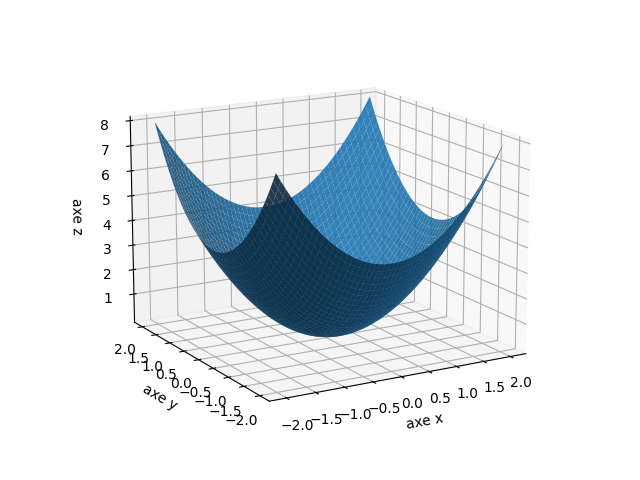
\includegraphics[scale=\myscale,scale=0.5]{figures/fonctions-extrem-1a}
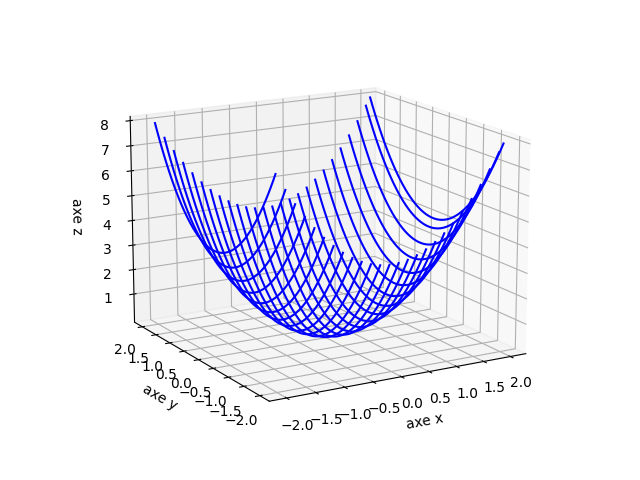
\includegraphics[scale=\myscale,scale=0.5]{figures/fonctions-extrem-1b}
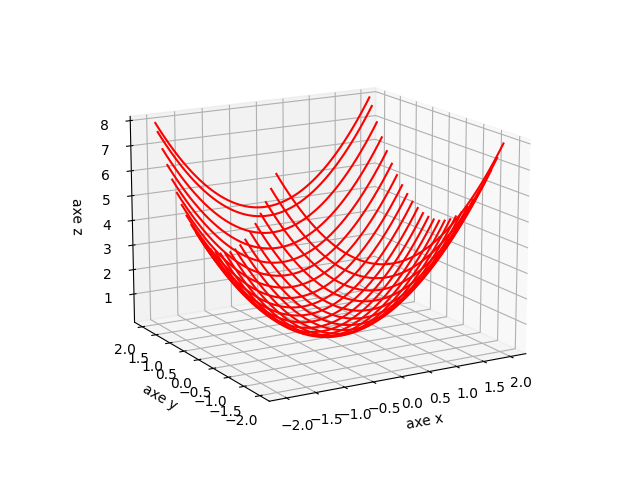
\includegraphics[scale=\myscale,scale=0.5]{figures/fonctions-extrem-1c}
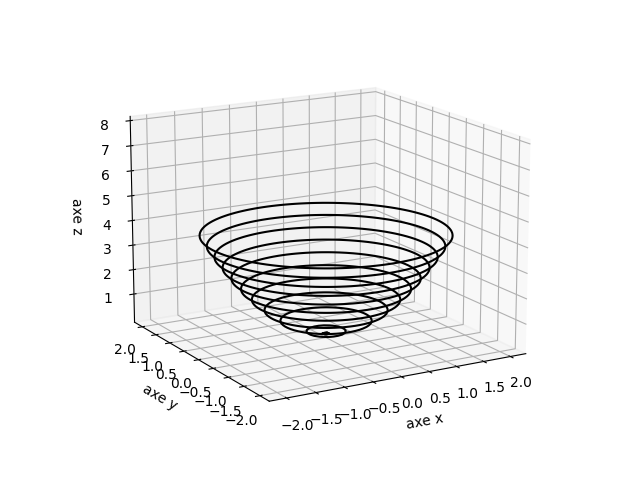
\includegraphics[scale=\myscale,scale=0.5]{figures/fonctions-extrem-1d}
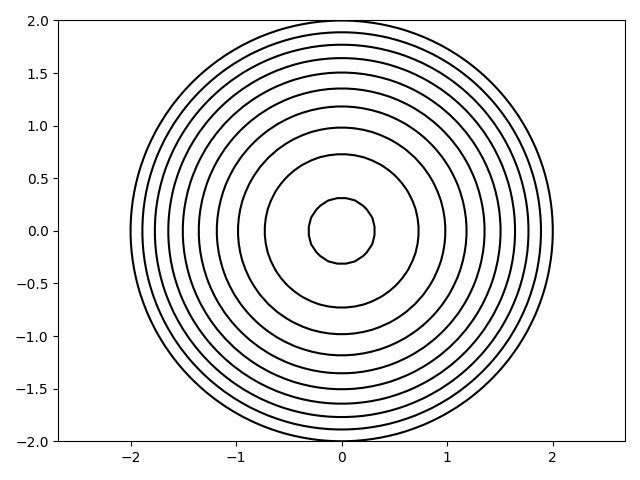
\includegraphics[scale=\myscale,scale=0.5]{figures/fonctions-extrem-1e}
\end{center}

% dessins 3d voir 'fonctions-extrem-1.py' 

\end{exemple}
	
\begin{exemple}
$f(x,y) = -x^2 - y^2$. C'est un exemple de maximum local atteint en $(0,0)$.


\begin{center}
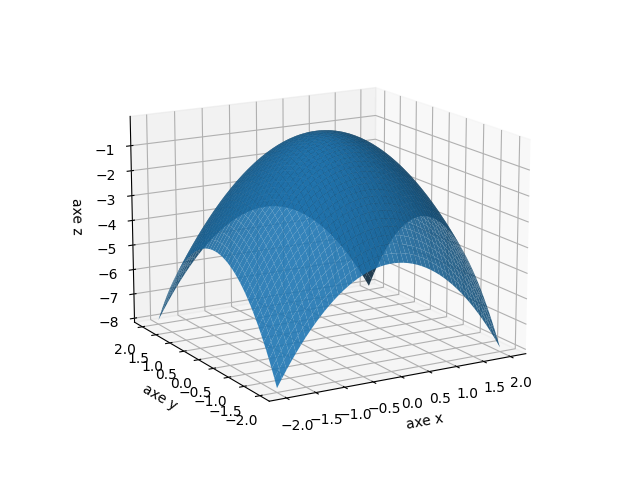
\includegraphics[scale=\myscale,scale=0.5]{figures/fonctions-extrem-2a}
\end{center}

% dessins 3d voir 'fonctions-extrem-2.py' 
	
\end{exemple}

\begin{exemple}
$f(x,y) = x^2 - y^2$. C'est un exemple de point-selle en $(0,0)$.

\begin{itemize}
  \item Les tranches sont des paraboles, tournées vers le haut ou vers le bas selon la direction de la tranche.
  \item Les lignes de niveau sont des hyperboles.
  \item Le graphe est donc un \defi{paraboloïde hyperbolique} que l'on appelle aussi la \defi{selle de cheval}\index{point-selle}.
  \item Un autre nom pour cette surface est un \defi{col} (en référence à un col en montagne). 
  En effet, le point $(0,0,0)$ est le point de passage le moins haut pour passer d'un versant à l'autre de la montagne. 
\end{itemize}

Ci-dessous : (a) la surface, (b) les tranches avec $x$ constant, (c) les tranches avec $y$ constant, (d) les courbes de niveau, (e) les lignes de niveau dans le plan (en pointillé les lignes de niveau négatif).
\begin{center}
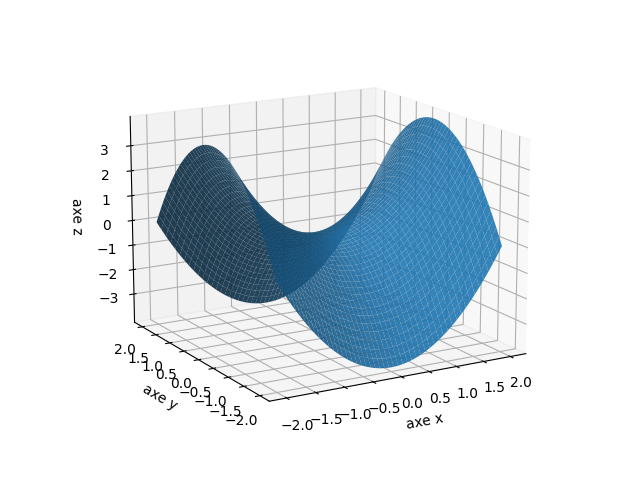
\includegraphics[scale=\myscale,scale=0.5]{figures/fonctions-extrem-3a}
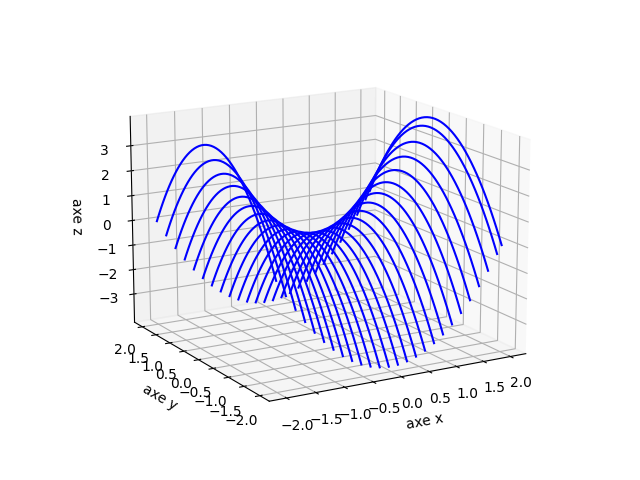
\includegraphics[scale=\myscale,scale=0.5]{figures/fonctions-extrem-3b}
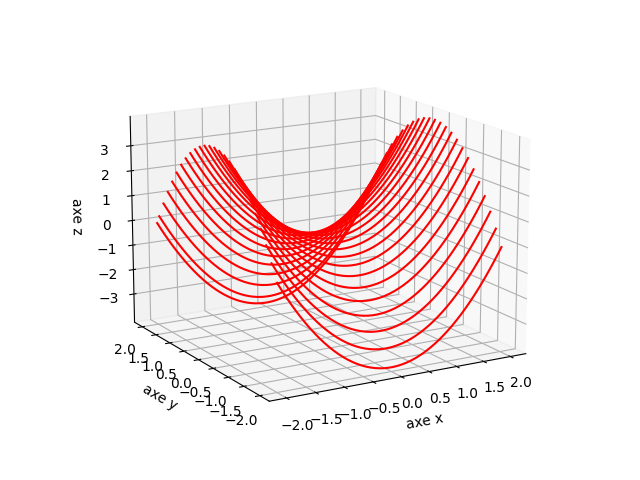
\includegraphics[scale=\myscale,scale=0.5]{figures/fonctions-extrem-3c}
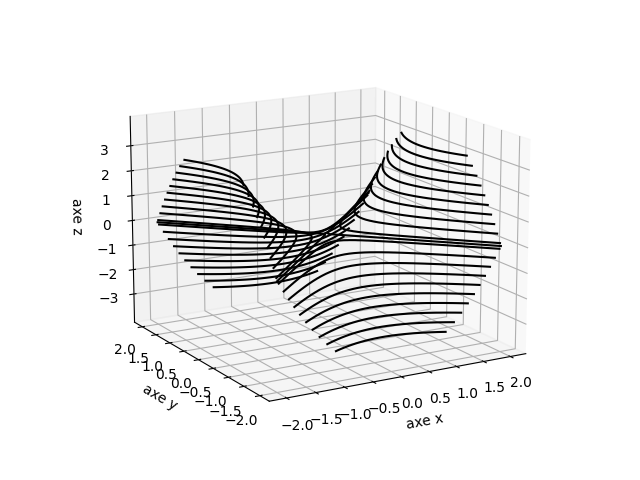
\includegraphics[scale=\myscale,scale=0.5]{figures/fonctions-extrem-3d}
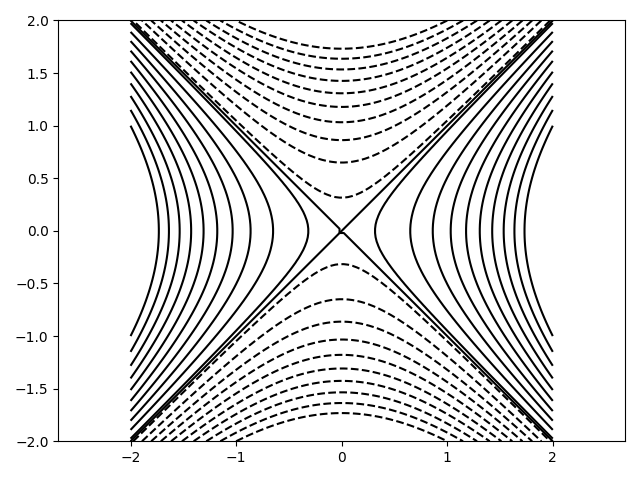
\includegraphics[scale=\myscale,scale=0.5]{figures/fonctions-extrem-3e}
\end{center}

% dessins 3d voir 'fonctions-extrem-3.py' 	
\end{exemple}





%----------------------------------------------------
\subsection{Caractérisation des minimums et maximums}

Pour une fonction $f : \Rr^2 \to \Rr$, nous utiliserons la notation de Monge, qui fournit un critère simple pour détecter un minimum ou un maximum local.
\begin{theoreme}[Critère de Monge]
Soit $f : \Rr^2 \to \Rr$ une fonction de classe $\mathcal{C}^2$ et soit $(x_0,y_0)$ un point critique de $f$.
 On pose 
$$
	r=\frac{\partial^2 f}{\partial x^2}(x_0,y_0)  
	\qquad 
	s=\frac{\partial^2 f}{\partial x \partial y}(x_0,y_0)
	\qquad
	t=\frac{\partial^2 f}{\partial y^2}(x_0,y_0).
$$
Alors :
\begin{itemize}
	\item si $rt-s^2>0$ et $r>0$, alors $(x_0,y_0)$ est un minimum local de $f$,
	\item si $rt-s^2>0$ et $r<0$, alors $(x_0,y_0)$ est un maximum local de $f$,
	\item si $rt-s^2<0$, alors $(x_0,y_0)$ n'est ni un minimum local ni un maximum local : c'est un point-selle,
	 \item si $rt-s^2=0$, on ne peut pas conclure directement (il faut approfondir l'étude).
\end{itemize}
\end{theoreme}

Remarque : $rt-s^2$ est le déterminant de la matrice hessienne en $(x_0,y_0)$, $H_f(x_0,y_0) = \begin{pmatrix}r&s\\s&t\end{pmatrix}$.

\begin{exemple}
Reprenons les trois exemples fondamentaux, pour vérifier notre critère.
\begin{enumerate}
	\item Soit  $f(x,y)=x^2+y^2$. Le point $(0,0$) est l'unique point critique de $f$.
On calcule 
$$r=\frac{\partial^2 f}{\partial x^2}(0,0)=2 
\qquad 
s=\frac{\partial^2 f}{\partial x \partial y}(0,0)=0
\qquad
t=\frac{\partial^2 f}{\partial y^2}(0,0)=2.$$
Ainsi, $rt-s^2 = 4$ avec $r>0$, et donc $(0,0)$ est bien un minimum local de $f$.
  \item Exercice : faire le même travail avec $f(x,y)=-x^2-y^2$. 
  \item Soit $f(x,y)=x^2-y^2$. On trouve un seul point critique : $(0,0)$. 
   On calcule $H_f(0,0) = \left(\begin{smallmatrix}2&0\\0&-2\end{smallmatrix}\right)$.
   Cette fois, $r=2$, $s=0$, $t=-2$. Ainsi, $rt-s^2 = -4 < 0$ et donc $(0,0)$ correspond bien à un point-selle.
\end{enumerate}

\end{exemple}


%----------------------------------------------------
\subsection{Autres exemples}

\begin{exemple}
Soit $f: \Rr^2 \to \Rr$ définie par $f(x,y)=x^3+y^3-3xy$.


\begin{center}
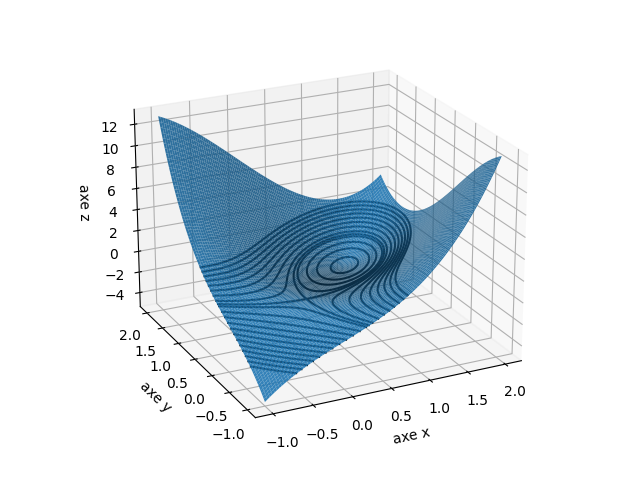
\includegraphics[scale=\myscale,scale=0.8]{figures/fonctions-extrem-4}
\end{center}

% dessins 3d voir 'fonctions-extrem-4.py' 
	

\begin{itemize}
	\item \textbf{Dérivées partielles.}
    $$\frac{\partial f}{\partial x}(x,y) = 3x^2-3y \qquad\qquad
    \frac{\partial f}{\partial y}(x,y) = 3y^2-3x$$
    	
	\item \textbf{Points critiques.}
    Ce sont les points où $\frac{\partial f}{\partial x}(x,y) = 0$ et $\frac{\partial f}{\partial y}(x,y) = 0$ en même temps. On a donc simultanément $x^2=y$ et $y^2=x$ (ce qui implique $x,y\ge0$).
    D'où $x^4 = y^2 = x$ dont les solutions positives sont $x=0$ (et alors $y=0$) et $x=1$ (et alors $y=1$). Ainsi, les points critiques sont $(0,0)$ et $(1,1)$.
	
	\item \textbf{Dérivées partielles secondes.}
    $$\frac{\partial^2 f}{\partial x^2}(x,y) = 6x
    \qquad 
    \frac{\partial^2 f}{\partial x \partial y}(x,y) = -3
    \qquad
    \frac{\partial^2 f}{\partial y^2}(x,y) = 6y$$
	
	\item \textbf{Étude en $(0,0)$.}     
    $$H_f(0,0) = \begin{pmatrix}0&-3\\-3&0\end{pmatrix}$$
    C'est-à-dire $r=0$, $s=-3$, $t=0$, donc $rt-s^2 = -9 < 0$ et donc $(0,0)$ est un point-selle.
   
	
    \item \textbf{Étude en $(1,1)$.}	
    $$H_f(1,1) = \begin{pmatrix}6&-3\\-3&6\end{pmatrix}$$
    C'est-à-dire $r=6$, $s=-3$, $t=6$, donc $rt-s^2 = 27 > 0$ avec $r>0$ et donc $(1,1)$ est un point de minimum de $f$ (c'est un minimum local et pas global).	
\end{itemize}

\end{exemple}

\bigskip	

Voici un exemple où le critère ne permet pas de conclure. Il faut terminer l'étude à la main.
\begin{exemple}
Soit $f(x,y)=2x^3-y^4-3x^2$. On trouve deux points critiques : $(0,0)$ et $(1,0)$. Par ailleurs :
$$H_f(0,0)=\begin{pmatrix}-6&0\\ 0&0\end{pmatrix}\qquad \text{ et } \qquad H_f(1,0)=\begin{pmatrix}6&0\\ 0&0\end{pmatrix}.$$
On ne peut pas conclure car le déterminant $rt-s^2$ est nul. On étudie chaque cas à la main.


\begin{center}
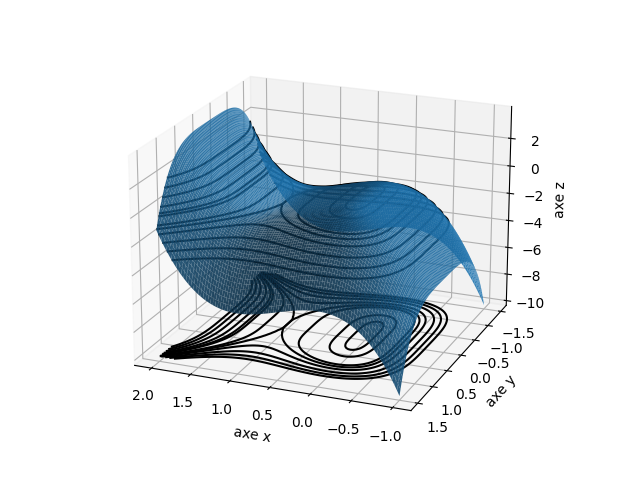
\includegraphics[scale=\myscale,scale=0.8]{figures/fonctions-extrem-5}
\end{center}

% dessins 3d voir 'fonctions-extrem-5.py' 

\begin{itemize}
	\item En $(0,0)$. 
	Écrivons $f(x,y)=x^2(2x-3)-y^4$.
	Pour $|x|\le 1$, on a $2x-3 \le0$, et donc 
	$$f(x,y)=x^2(2x-3)-y^4 \le 0.$$
	Comme $f(0,0)=0$, alors $f$ admet un maximum local au point $(0,0)$.
	
	\item  En $(1,0)$. 
	Tout d'abord, on se limite aux points de la forme $(1,y)$ (autour de $y_0=0$) :
		$$f(1,y)=-1-y^4\le -1 = f(1,0)$$
		
	Ensuite, on se limite aux points de la forme $(x,0)$ (autour de $x_0=1$, par exemple pour $x$ tel que  $|x-1|\leq 1$) : 
	$$ f(x,0)=(x-1)^2(2x+1)-1 \ge -1 = f(1,0)$$
	Donc, en $(1,0)$, ce n'est ni un minimum ni un maximum : c'est un point-selle.
	
\end{itemize}

\end{exemple}




%----------------------------------------------------
\subsection{Valeurs propres de la hessienne}

Ce paragraphe peut être omis à la première lecture.

Nous reformulons le critère précédent en termes de valeurs propres de la matrice hessienne.
Les valeurs propres de la matrice $H_f(x_0,y_0)$ sont les racines du polynôme caractéristique qui est défini par $\chi(\lambda)=\det \left( H_f(x_0,y_0)-\lambda I \right)$.

\begin{theoreme}
Soient $U$ un ouvert de $\Rr^2$, $f$ une fonction de classe $\mathcal{C}^2$ sur $U$ et $(x_0,y_0)\in U$ un point critique de $f$.
\begin{enumerate}
    \item Si $H_f(x_0,y_0)$ a ses deux valeurs propres strictement positives, alors $f$ présente un minimum en $(x_0,y_0)$.
    \item Si $H_f(x_0,y_0)$ a ses deux valeurs propres strictement négatives, alors $f$ présente un maximum en $(x_0,y_0)$.
    \item Si $H_f(x_0,y_0)$ a deux valeurs propres de signes opposés, alors $f$ ne présente pas d'extremum en $(x_0,y_0)$ : c'est un point-selle.
    \item Dans les autres cas, on ne peut rien dire (tout peut arriver).
\end{enumerate}
\end{theoreme}


%----------------------------------------------------
\begin{miniexercices}
    \sauteligne
    \begin{enumerate}
        \item Soit $f(x,y)=\exp(-\frac 13 x^3 + x - y^2)$. Déterminer les deux points critiques de $f$ et la nature (minimum/maximum/point-selle) de chacun d'entre eux.

\begin{center}
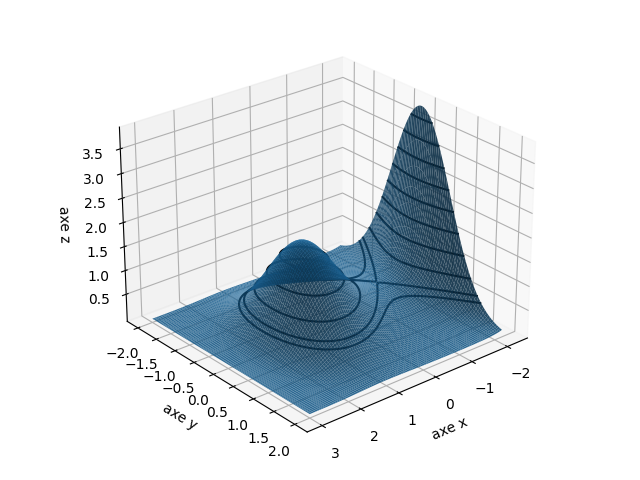
\includegraphics[scale=\myscale,scale=0.6]{figures/fonctions-extrem-7}
\end{center}

% dessins 3d voir 'fonctions-extrem-7.py' 


        \item Soit $f(x,y)=x^3-3xy^2$. Déterminer le point critique de $f$ et sa nature.
        Le graphe de $f$ s'appelle une \og{}selle de singe\fg{}.

\begin{center}
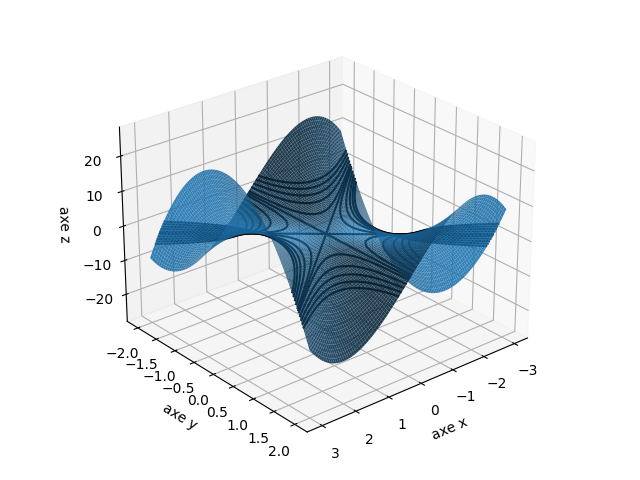
\includegraphics[scale=\myscale,scale=0.6]{figures/fonctions-extrem-6}
\end{center}

% dessins 3d voir 'fonctions-extrem-6.py' 
        
        \item Soit $f(x,y)=x^4+y^4-2x^2$. Déterminer les trois points critiques de $f$.
        Le critère de Monge permet-il de conclure ?
        Déterminer quand même la nature de chacun de ces points critiques.

%On trouve trois points critiques $(-1,0)$, $(1,0)$ et $(0,0)$. Par ailleurs,
%        $$H_f(-1,0)=H_f(1,0)=\left(\begin{array}{cc}8&0\\ 0&0\end{array}\right)\quad \mbox{ et }\quad H_f(0,0)=\left(\begin{array}{cc}-4&0\\ 0&0\end{array}\right).$$
%        On ne peut pas conclure. Or
%        $$f(x,y)=(x^2-1)^2+y^4-1\geq -1=f(\pm 1,0).$$
%        Donc $f$ admet un minimum aux points $(\pm 1,0)$. D'autre part, pour $|x|\leq 1$,
%        $$f(x,0)=x^4-2x^2=x^2(x^2-2)\leq 0=f(0,0)\quad \mbox{ et }\quad f(0,y)=y^4\geq 0=f(0,0).$$
%        Donc $(0,0)$ n'est ni un maximum ni un minimum ; c'est un point selle.


    \end{enumerate}
\end{miniexercices}

 


%%%%%%%%%%%%%%%%%%%%%%%%%%%%%%%%%%%%%%%%%%%%%%%%%%%%%
\section{Minimum et maximum : cas général}

Nous étendons les résultats précédents dans deux directions : tout d'abord pour les fonctions avec un nombre quelconque de variables, puis pour la recherche de minimums/maximums sur un compact.


%----------------------------------------------------
\subsection{Cas de $\Rr^n$}

Soit $n\ge2$.
Étendons les définitions au cas d'une fonction $f : U\to \Rr$, o\`u $U$ est un ouvert de $\Rr^n$.

\begin{itemize}
    \item $f$ admet un \defi{maximum local} (resp. \defi{minimum local}) en $x_0 \in U$ s'il existe une boule ouverte $B\subset U$ centrée en $x_0$ telle que, 
    pour tout $x \in B$, on ait $f(x) \le f(x_0)$ (resp. $f(x) \ge f(x_0)$).
        
    \item $f$ admet un \defi{extremum local} en $x_0$ si elle y admet un maximum local ou un minimum local.
    
    \item $x_0$ est un \defi{point critique} de $f$ si le gradient de $f$ s'annule en $x_0$, ou autrement dit si $\frac{\partial f}{\partial x_i}(x_0) = 0$ pour tout $i=1,\ldots,n$. 
      
    \item  \textbf{Proposition.} Si $f$ admet un extremum local en $x_0 \in U$ et si le gradient est défini en ce point, alors $x_0$ est un point critique de $f$.

    \item Ainsi, on cherche les extremums locaux parmi les points critiques de $f$.
\end{itemize}


    
    
%----------------------------------------------------
\subsection{Extremum sur un compact}

Pour une fonction  d'une variable $f : [a,b] \to \Rr$ continue sur un intervalle compact, on sait que $f$ est bornée et atteint ses bornes, c'est-à-dire qu'elle atteint un minimum global et atteint aussi un maximum global.  Ce minimum ou ce maximum peut être atteint au \og{}bord\fg{} du segment, c'est-à-dire en $a$ ou en $b$, ou bien à \og{}l'intérieur\fg{} $]a,b[$. 
Il faut faire attention à bien distinguer l'étude à l'intérieur et au bord. En effet, à l'intérieur, un extremum est un point critique de $f$, alors que sur le bord ce n'est plus nécessairement le cas. Garder en mémoire l'exemple $f(x) = x^2$ sur $[-1,1]$ : la dérivée s'annule en $x=0$ (minimum local et global) mais un maximum (local et global) est atteint en $x=1$ et $x=-1$ alors que la dérivée ne s'y annule pas (explication : $+1$ et $-1$ sont au bord de l'intervalle).


\myfigure{1}{
    \tikzinput{fig-extrem-07}     
}



Cette propriété se généralise aux fonctions de plusieurs variables, continues sur un ensemble compact. (Nous l'admettons.)

\begin{proposition}
Soit $f : K \rightarrow \Rr$ une fonction continue sur un ensemble compact $K \subset \Rr^n$. Alors $f$ est bornée et atteint ses extremums sur $K$.
\end{proposition}

La marche à suivre pour étudier les extremums d'une fonction différentiable sur un compact $K \subset \Rr^n$ est la suivante :
\begin{enumerate}
    \item Rechercher les points critiques dans l'intérieur de $K$.
    \item Déterminer si chacun de ces points critiques est un maximum local, un minimum local ou ni l'un ni l'autre. (Dans le cas $n=2$, on utilise les dérivées partielles secondes. Il existe des généralisations de ces formules à $n$ quelconque.)
    \item Chercher si $f$ admet des extremums sur le bord de $K$ (le critère des points critiques n'est plus valable).
    \item Comparer les minimums pour déterminer le -- ou les -- minimums globaux  ; idem pour les maximums.
\end{enumerate}

On rappelle qu'un ensemble $A \subset \Rr^n$ découpe l'espace en trois parties disjointes : son intérieur $\operatorname{Int} A$, son bord $\partial A$ (ou frontière), et son extérieur $\operatorname{Ext} A$.


\myfigure{1}{
    \tikzinput{fig-extrem-08}     
}



\begin{exemple}
Déterminons les extremums de $f$ sur $K$ où :
$$f(x,y) = x^2 - y^2 \qquad \text{ et } \qquad K = \lbrace (x,y) \in \Rr^2  \mid  x^2 + y^2 \leq 1 \rbrace.$$

\myfigure{1}{
    \tikzinput{fig-extrem-09}     
}


On procède de la manière suivante :     
\begin{enumerate}
    \item On cherche les points critiques et les extremums locaux dans $\operatorname{Int} K$.
    On trouve un seul point critique, en $(0,0)$. Mais, en $(0,0)$, $f$ a un point-selle. La fonction n'a donc pas d'extremum à l'intérieur de $K$. Mais comme $K$ est compact et $f$ est continue sur $K$, $f$ est bornée sur $K$ et atteint ses bornes sur $K$. Ce sera donc sur le bord de $K$.
    
    \item On analyse $f$ sur $\partial K$.
    Une possibilité ici est de paramétrer le bord de $K$ : c'est le cercle de rayon $1$ centré en $(0,0)$ que l'on paramètre par $(\cos t,\sin t)$, pour $t\in[0,2\pi]$. On obtient :
    $f(\cos t,\sin t)=\cos^2t-\sin^2t=\cos(2t)$. On peut alors étudier les variations de cette fonction. On obtient qu'elle est maximum, égale à $1$, lorsque $2t \equiv 0 \pmod{2\pi}$, et minimum, égale à $-1$, lorsque $2t \equiv \pi \pmod{2\pi}$. La fonction $f$ atteint donc son maximum $1$ aux points $(1,0)$ et $(-1,0)$ de $K$, et son minimum $-1$ aux points $(0,1)$ et $(0,-1)$.
\end{enumerate}

\begin{center}
  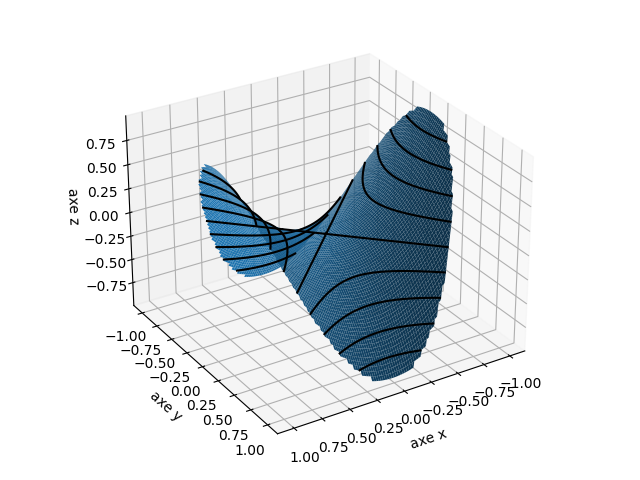
\includegraphics[scale=\myscale,scale=0.6]{figures/fonctions-extrem-8}
\end{center}

\end{exemple}



%----------------------------------------------------
\begin{miniexercices}
    \sauteligne
    \begin{enumerate}
        \item Déterminer les extremums (locaux et globaux) de $f(x,y) = x^2+y^2$ sur $C = [-1,1] \times [-1,1]$. Même question avec $f(x,y)= xy$.

        \item Déterminer les extremums (locaux et globaux) de $f(x,y) = x^3-y^2$ sur $D = \lbrace (x,y) \in \Rr^2  \mid  x^2 + y^2 \leq 1 \rbrace$.

        \item Déterminer les extremums (locaux et globaux) de $f(x,y) = y\cos(x)$ sur $B = \Rr \times [0,1]$.
    \end{enumerate}
\end{miniexercices}



%%%%%%%%%%%%%%%%%%%%%%%%%%%%%%%%%%%%%%%%%%%%%%%%%%%%%
\section{Extremums liés}

Dans cette section, nous allons nous intéresser à la recherche des extremums sous certaines contraintes.

Vous savez que le mont Blanc culmine à 4807 mètres. Mais si vous randonnez autour du mont Blanc, quelle sera votre altitude maximale selon le parcours que vous effectuez ?

%----------------------------------------------------
\subsection{Extremums liés dans le plan}

Commençons par les fonctions de deux variables. 

Problème : trouver le maximum (ou le minimum) d'une fonction $f(x,y)$ sachant que $(x,y)$ doit vérifier $g(x,y)=0$.

Exemple : trouver le minimum de $f(x,y) = x^2 + 2y^2$ avec la contrainte $y = 2x-1$ (c'est-à-dire $g(x,y)=0$ avec $g(x,y)=y-2x+1$ par exemple).

Clairement, le minimum global de $f$ est $0$, atteint en $(0,0)$, mais ce point ne vérifie pas la contrainte $g(x,y)=0$.

Géométriquement, il s'agit de trouver le minimum de $f(x,y)$ en se limitant aux points $(x,y)$ du plan situés sur la droite d'équation $y=2x-1$.
Sur les figures ci-dessous : la surface\couleurnb{ bleue}{} est le graphe de $f$, la droite\couleurnb{ rouge}{} est l'ensemble $(g(x,y)=0)$. La contrainte impose de ne considérer que des points $(x,y,z)$ au-dessus de cette droite : ils sont donc ici sur la courbe\couleurnb{ orange}{} tracée sur la surface.
Trouver le minimum de $f$ avec cette contrainte, c'est trouver le point $(x,y,z)$ de la courbe\couleurnb{ orange}{} ayant une altitude $z$ minimale. 

\begin{center}
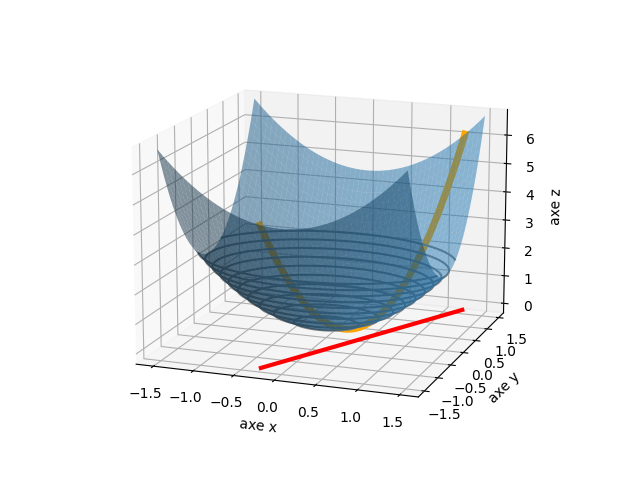
\includegraphics[scale=\myscale,scale=0.7]{figures/fonctions-extremlie-1a}

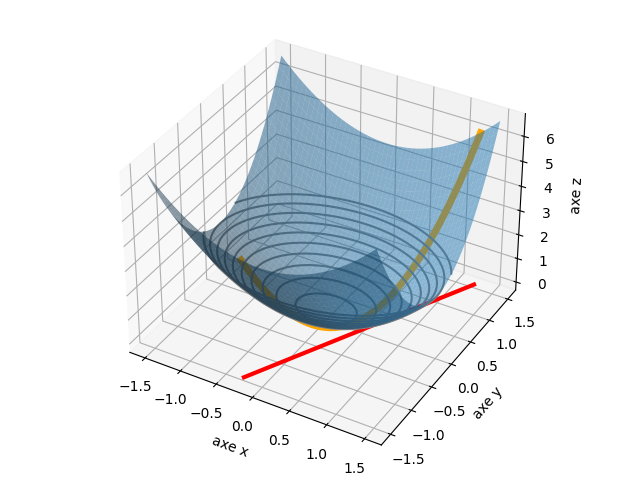
\includegraphics[scale=\myscale,scale=0.5]{figures/fonctions-extremlie-1b}
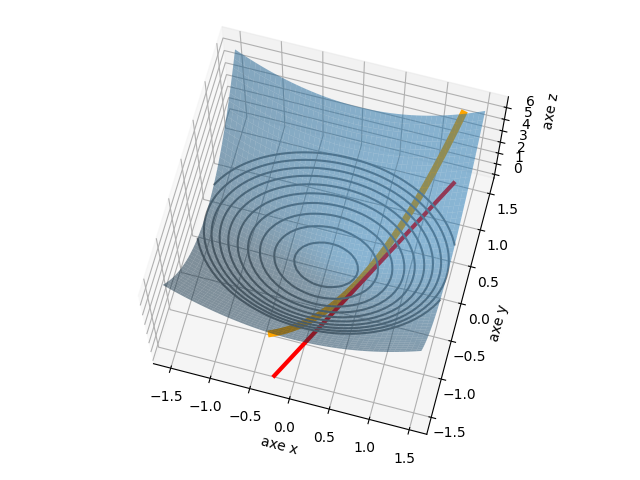
\includegraphics[scale=\myscale,scale=0.5]{figures/fonctions-extremlie-1c}
\end{center}

% dessins 3d voir 'fonctions-extremlie-1.py' 	


\begin{theoreme}[Extremums liés -- Deux variables]
Soient $f,g: U \to \Rr$ des fonctions de classe $\mathcal{C}^1$ sur un ouvert $U$ de $\Rr^2$.
Soit $(x_0,y_0) \in U$ tel que $f$ soumise à la contrainte $g(x,y)=0$ admette un extremum au point $(x_0,y_0)$
et $\grad g(x_0,y_0) \neq (0,0)$.
Alors il existe un nombre réel $\lambda$ tel que 
$\grad f(x_0,y_0) = \lambda \grad g(x_0,y_0).$
Autrement dit, on a :
$$
\left\{
\begin{array}{rcl}
g(x_0,y_0) & = & 0 \\[1ex]
\dfrac{\partial f}{\partial x}(x_0,y_0) &=& \lambda \dfrac{\partial g}{\partial x}(x_0,y_0) \\[1ex]
\dfrac{\partial f}{\partial y}(x_0,y_0) &=& \lambda \dfrac{\partial g}{\partial y}(x_0,y_0) \\ 
\end{array}\right.
$$
\end{theoreme}

Noter qu'on peut aussi considérer la contrainte $g(x,y)=c$ (où $c$ est une constante), qui se ramène au cas énoncé dans le théorème en considérant $g(x,y)-c=0$.

\textbf{Interprétation géométrique.}
En un extremum lié $(x_0,y_0)$, les gradients de $f$ et $g$ sont colinéaires. Cela signifie que la courbe $(f(x,y) = c_0)$ (avec $c_0 = f(x_0,y_0)$) et la courbe $(g(x,y)=0)$ ont la même tangente au point $(x_0,y_0)$. Autrement dit, ces deux courbes sont tangentes entre elles.

\myfigure{1}{
    \tikzinput{fig-extremlie-01}     
}


\textbf{Remarque sur les équations.} Le théorème des extremums liés en dimension $n$ quelconque conduit à un système de $n$ équations à $n$ inconnues. Mais attention ! Les équations ne sont pas linéaires. Ainsi, le système obtenu est généralement très difficile voire impossible à résoudre, même pour des situations simples. C'est pourquoi les fonctions que l'on étudiera dans la suite sont toutes très simples, afin de pouvoir résoudre les équations.



\begin{exemple}
Reprenons l'exemple illustré précédemment : trouver le minimum de $f(x,y) = x^2 + 2y^2$ avec la contrainte $y = 2x-1$.

Géométriquement, on cherche le point situé sur la droite d'équation $y = 2x-1$ qui minimise la fonction $f$.

On pose $g(x,y) = y - 2x+1$.
$$\grad f(x,y) = \begin{pmatrix} 2x \\ 4y \end{pmatrix}
\qquad \grad g(x,y) = \begin{pmatrix} -2 \\ 1 \end{pmatrix}.$$
En un extremum lié, les gradients sont colinéaires : $\grad f(x,y) = \lambda \grad g(x,y)$.
On obtient deux équations :
\begin{align}
2x &= -2\lambda \label{eqex1}\\
4y &= \lambda \label{eqex2}
\end{align}
auxquelles on rajoute la contrainte $g(x,y) = 0$ :
\begin{equation}
y = 2x-1
\label{eqex3}
\end{equation}

Par \eqref{eqex1}, on obtient $x = -\lambda$, et par \eqref{eqex2}, on trouve $y = \frac\lambda4$, qu'on injecte dans \eqref{eqex3} :
$$\frac\lambda4 = -2\lambda - 1.$$
Ainsi, 
$$\lambda_0 = -\frac{4}{9}.$$
On obtient donc la solution :
$$(x_0,y_0) = \left( \frac{4}{9},  -\frac{1}{9} \right).$$

Sur $(g(x,y)=0)$, la fonction $f$ est positive et tend vers $+\infty$ lorsque $\|(x,y)\|$  tend vers $+\infty$, donc $f$ admet au moins un minimum. Conclusion : $f$ admet un unique minimum sur $(g(x,y)=0)$, et ce minimum est atteint en $(x_0,y_0)$.

Géométriquement, les courbes $(f(x,y)=k)$ sont des ellipses, que l'on fait grandir jusqu'à obtenir l'ellipse tangente à la droite. Le point de contact est le point recherché.

\myfigure{1}{
    \tikzinput{fig-extremlie-02}     
}

\end{exemple}


\begin{exemple}
Quel est le point de la parabole définie par $y = -x^2$ le plus proche du point $(2,1)$ ?


\myfigure{0.8}{
    \tikzinput{fig-extremlie-03bis}     
}

On pose $f(x,y) = (x-2)^2+(y-1)^2$ qui mesure la distance (au carré) entre le point $(x,y)$ et le point $(2,1)$. La contrainte est donnée par 
$g(x,y) = 0$ où $g(x,y) = y+x^2$. 

$$\grad f(x,y) = \begin{pmatrix} 2(x-2) \\ 2(y-1) \end{pmatrix}
\qquad \grad g(x,y) = \begin{pmatrix} 2x \\ 1 \end{pmatrix}.$$
En un extremum lié, les gradients sont colinéaires : $\grad f(x,y) = \lambda \grad g(x,y)$. Donc :
\setcounter{equation}{0}
\begin{align}
2(x-2) &= 2\lambda x  \label{eqexx1}\\
2(y-1) &= \lambda \label{eqexx2}
\end{align}
On rajoute la contrainte $g(x,y) = 0$ :
\begin{equation}
y+x^2 = 0
\label{eqexx3}
\end{equation}

Par \eqref{eqex1}, on a $x = \frac{2}{1-\lambda}$, et par \eqref{eqex2}, on a $y = \frac\lambda2+1$, qu'on injecte dans \eqref{eqex3} :
$$\frac\lambda2+1 + \frac{4}{(1-\lambda)^2} = 0.$$
Cette dernière équation est équivalente à :
$$(\lambda+2) (\lambda-1)^2 + 8 =0,$$
qui sous forme développée est $\lambda^3-3\lambda+10=0$.
C'est une équation de degré $3$, qui ici admet une seule solution réelle (loin d'être évidente) :
$$\lambda_0 = \frac{-1-\left(\sqrt[3]{5-2\sqrt6}\right)^2}{\sqrt[3]{5-2\sqrt6}}$$

On obtient donc la solution :
$$(x_0,y_0) = \left( \frac{2}{1-\lambda_0},  \frac{\lambda_0}2+1 \right).$$


% [x == 0.5535737878187343, y == -0.3064439140811456, lambda == -2.612887828162291]


Approximations numériques :  $\lambda_0 \simeq -2.613$ et $(x_0,y_0) \simeq (0.554,-0.306)$.

Interprétation géométrique. On fait grandir un cercle centré à l'origine jusqu'à ce qu'il soit tangent à la parabole. Le point de contact obtenu correspond à la distance minimale. En augmentant encore le rayon, on pourrait obtenir d'autres extremums liés (mais ce n'est pas le cas ici).  

\myfigure{1}{
    \tikzinput{fig-extremlie-03}     
}


\end{exemple}


%----------------------------------------------------
\subsection{Extremums liés avec une seule contrainte}

Passons au cas d'un nombre quelconque de variables, mais toujours avec une seule contrainte.
Il s'agit de trouver les extremums de $f(x)$ lorsque $x$ appartient à une hypersurface définie par $g(x) = 0$.

Exemple : trouver le minimum de $f(x,y,z) = x^2 + y^2 + z^2$ avec la contrainte $x + 2y +3z = 1$.

\begin{theoreme}[Extremums liés -- Une contrainte]
Soient $f,g: U \to \Rr$ des fonctions de classe $\mathcal{C}^1$ sur un ouvert $U$ de $\Rr^n$.
Soit $x_0 \in U$ tel que $f$ soumise à la contrainte $g(x)=0$ admette un extremum au point $x_0$ et $\grad g(x_0) \neq 0$.
Alors il existe un nombre réel $\lambda$ tel que $\grad f(x_0) = \lambda \grad g(x_0).$
\end{theoreme}

Le réel $\lambda$ est appelé \defi{multiplicateur de Lagrange}.

\begin{remarque*}
Si $x_0$ est un extremum lié, on a $\grad f(x_0)$ colinéaire à $\grad g(x_0)$.
La réciproque n'est pas vraie. Nous avons une condition nécessaire mais pas suffisante. C'est l'équivalent de la nullité de la dérivée pour les extremums libres : en un extremum libre la dérivée est nulle, mais la dérivée peut être nulle sans que la fonction ait un extremum (penser à $x\mapsto x^3$ en $x=0$).  
\end{remarque*}


\begin{exemple}
Trouver le minimum de $f(x,y,z) = x^2 + y^2 + z^2$ avec la contrainte $x + 2y +3z = 1$.


Géométriquement, on cherche le point, situé sur le plan d'équation $x + 2y +3z = 1$, qui est le plus proche de l'origine.


On pose $g(x,y,z) = x + 2y +3z - 1$.
$$\grad f(x,y,z) = \begin{pmatrix} 2x \\ 2y \\ 2z \end{pmatrix}
\qquad \grad g(x,y,z) = \begin{pmatrix} 1 \\ 2 \\ 3 \end{pmatrix}.$$
En un extremum lié, les gradients sont colinéaires : $\grad f(x,y,z) = \lambda \grad g(x,y,z)$.
On obtient trois équations
\setcounter{equation}{0}
\begin{align}
2x &= \lambda \label{eqexxx1}\\
2y &= 2\lambda \label{eqexxx2}\\
2z &= 3\lambda \label{eqexxx3}
\end{align}
auxquelles on rajoute la contrainte $g(x,y,z) = 0$ :
\begin{equation}
x + 2y +3z = 1
\label{eqexxx4}
\end{equation}
Par \eqref{eqexxx1}, on a $x = \frac12\lambda$, par \eqref{eqexxx2}, on a $y = \lambda$, et par \eqref{eqexxx3}, on a $z = \frac32\lambda$, qu'on injecte dans \eqref{eqexxx4} :
$$\frac12\lambda + 2\lambda + \frac92\lambda = 1.$$
Ainsi, 
$$\lambda_0 = \frac{1}{7} \qquad \text{ et } \qquad (x_0,y_0,z_0) = \left( \frac{1}{14},  \frac{1}{7}, \frac{3}{14} \right).$$

Sur $(g(x,y,z)=0)$, la fonction $f$ est positive et tend vers $+\infty$ lorsque $\|(x,y,z)\|$ tend vers $+\infty$, donc $f$ admet au moins un minimum.
Conclusion : $f$ admet un unique minimum sur $(g(x,y,z)=0)$, et ce minimum est atteint en $(x_0,y_0,z_0)$.
\end{exemple}


\begin{exemple}
Trouver les extremums de $f(x,y,z) = x + 2y +3z$ avec la contrainte $x^2 + y^2 + z^2 = 1$.

Géométriquement, on cherche les points situés sur la sphère de rayon $1$ centrée à l'origine qui minimisent ou maximisent la fonction $f$. Comme la sphère est un ensemble compact (et $f$ est continue), on sait que le minimum et le maximum seront atteints.


On pose $g(x,y,z) = x^2 + y^2 + z^2 - 1$.

$$\grad f(x,y,z) = \begin{pmatrix} 1 \\ 2 \\ 3 \end{pmatrix}
\qquad \grad g(x,y,z) = \begin{pmatrix} 2x \\ 2y \\ 2z \end{pmatrix}.$$
En un extremum lié, on a $\grad f(x,y,z) = \lambda \grad g(x,y,z)$ :
\setcounter{equation}{0}
\begin{align}
1 &= 2\lambda x \label{eqexxxx1}\\
2 &= 2\lambda y \label{eqexxxx2}\\
3 &= 2\lambda z\label{eqexxxx3}
\end{align}
On a de plus $g(x,y,z) = 0$ :
\begin{equation}
x^2 + y^2 + z^2 = 1
\label{eqexxxx4}
\end{equation}
D'une part, grâce à \eqref{eqexxxx1}, \eqref{eqexxxx2}, \eqref{eqexxxx3} :
$$(2\lambda x)^2 + (2\lambda y)^2 + (2\lambda z)^2 = 1^2+2^2+3^2 = 14.$$
D'autre part, grâce à \eqref{eqexxxx4} :
$$(2\lambda x)^2 + (2\lambda y)^2 + (2\lambda z)^2 = 4\lambda^2.$$
Ainsi, 
$$\lambda  = \pm\frac12\sqrt{14}.$$

On obtient donc deux solutions :
$$(x_1,y_1,z_1) = \left( \frac{1}{\sqrt{14}}, \frac{2}{\sqrt{14}}, \frac{3}{\sqrt{14}}\right)
\qquad \text{ et } \qquad
(x_2,y_2,z_2) = \left( -\frac{1}{\sqrt{14}}, -\frac{2}{\sqrt{14}}, -\frac{3}{\sqrt{14}}\right).$$
L'une doit correspondre au maximum de $f$ (c'est clairement $(x_1,y_1,z_1)$) et l'autre au minimum de $f$ (c'est $(x_2,y_2,z_2)$).
\end{exemple}



%----------------------------------------------------
\subsection{Extremums liés avec plusieurs contraintes}

Généralisons la situation précédente en présence de $k$ contraintes.

\begin{theoreme}[Extremums liés -- Plusieurs contraintes]
Soient $f: U \to \Rr$ et $g_1,\ldots,g_k : U \to \Rr$ des fonctions de classe $\mathcal{C}^1$
sur un ouvert $U$ de $\Rr^n$.

Supposons que les vecteurs $\grad g_1(x),\ldots, \grad g_k(x)$  soient linéairement indépendants, pour tout $x$ de l'ensemble $S$ défini par $(g_1(x)=0,\ldots,g_k(x)=0)$.

Si $f$ admet un extremum lié sur $S$ en $x_0$ alors le vecteur $\grad f(x_0)$ est combinaison linéaire des vecteurs $\grad g_i(x_0)$ : il existe $\lambda_1,\ldots,\lambda_k$ tels que 
$$\grad f(x_0)=\lambda_1\grad g_1(x_0) + \cdots + \lambda_k \grad g_k(x_0).$$
\end{theoreme}

Les réels $\lambda_1,\ldots,\lambda_k$ sont appelés \defi{multiplicateurs de Lagrange}.

\begin{exemple}
Trouver le point $(x,y,z)$ le plus proche de l'origine vérifiant $z^2 = x^2 + y^2$ et $x + y -2z+1=0$.

On pose $f(x,y,z) = x^2 + y^2 + z^2$, $g_1(x,y,z)= x^2 + y^2 - z^2$ et $g_2(x,y,z) = x + y -2z+1$.
 
$$
\grad f(x,y,z) = \begin{pmatrix} 2x \\ 2y \\ 2z \end{pmatrix}
\qquad \grad g_1(x,y,z) = \begin{pmatrix} 2x \\ 2y \\ -2z \end{pmatrix}
\qquad \grad g_2(x,y,z) = \begin{pmatrix} 1 \\ 1 \\ -2 \end{pmatrix}
$$
En un extremum lié, $\grad f(x,y,z)$ est combinaison linéaire de $\grad g_1(x,y,z)$
et $\grad g_2(x,y,z)$ :
$$\grad f(x,y,z) = \lambda \grad g_1(x,y,z) + \mu \grad g_2(x,y,z).$$
On obtient trois équations
\setcounter{equation}{0}
\begin{align}
2x &= 2\lambda x + \mu \label{eqeex1}\\
2y &= 2\lambda y  + \mu     \label{eqeex2}\\
2z &= -2\lambda z - 2\mu \label{eqeex3}
\end{align}
auxquelles on rajoute les contraintes $g_1(x,y,z) = 0$ et $g_2(x,y,z) = 0$ :
\begin{align}
z^2 - x^2 - y^2 &= 0  \label{eqeex4}\\
x + y -2z+1 &= 0      \label{eqeex5}
\end{align}

Nous obtenons donc $5$ équations (non linéaires !) avec $5$ inconnues.
Après calculs, les solutions sont :
$$(x_1,y_1,z_1) = \left( \frac{1+\sqrt2}{2}, \frac{1+\sqrt2}{2}, \frac{2+\sqrt2}{2} \right)
\qquad \text{ et } \qquad
(x_2,y_2,z_2) = \left( \frac{1-\sqrt2}{2}, \frac{1-\sqrt2}{2}, \frac{2-\sqrt2}{2} \right).$$

Le point $(x_1,y_1,z_1)$ est un maximum lié de $f$, et  $(x_2,y_2,z_2)$ est un minimum lié.
Géométriquement, $z^2 = x^2+y^2$ est un cône, que l'on intersecte par le plan $x + y -2z+1=0$ pour obtenir une ellipse de l'espace (donc un ensemble compact). Nous avons calculé le point $(x_2,y_2,z_2)$ de cette ellipse le plus proche de l'origine.
\end{exemple}


%----------------------------------------------------
\begin{miniexercices}
    \sauteligne
    \begin{enumerate}
        \item Quelles sont les dimensions du rectangle de périmètre $16$ qui a l'aire la plus grande possible ?

        \item Trouver le point du cercle de rayon $1$ centré à l'origine le plus éloigné du point $(3,4)$. 

        \item Calculer la distance entre le point $(x_0,y_0,z_0)$ et le plan d'équation $ax+by+cz+d=0$.

        \item Le cylindre infini d'équation $x^2+y^2=4$ et le plan $x+2y+z=2$ se coupent en une ellipse. Quel est le point de cette ellipse le plus éloigné de l'origine ?
    \end{enumerate}
\end{miniexercices}



\auteurs{
\\
Arnaud Bodin.
D'après des cours de Abdellah Hanani (Lille), 
Goulwen Fichou et Stéphane Leborgne (Rennes),
Laurent Pujo-Menjouet (Lyon). 
Relu par Anne Bauval et Vianney Combet.
}


\finchapitre 
\end{document}


